%%%%%%   TIPO DE DOCUMENTO: Artículo   %%%%%%
\documentclass[letterpaper,11pt,twoside]{report}

\usepackage[spanish]{babel} %Idioma
\usepackage{graphicx} %Imágenes
\usepackage[utf8]{inputenc} %Acentos
\usepackage{hyperref} %Links
\usepackage{xspace}
\usepackage{subfigure}
\usepackage{subcaption}
\usepackage{booktabs}
\usepackage{listings}
\usepackage{verbatim}
\usepackage{amsmath, amssymb}
\usepackage{amsmath}
\usepackage[active]{srcltx}
\usepackage{amssymb}
\usepackage{amscd}
\usepackage{makeidx}
\usepackage{amsthm}
\usepackage{algpseudocode}
\usepackage{algorithm}
\renewcommand{\baselinestretch}{1}
\setcounter{page}{1}
\setlength{\textheight}{21.6cm}
\setlength{\textwidth}{14cm}
\setlength{\oddsidemargin}{1cm}
\setlength{\evensidemargin}{1cm}
\pagestyle{myheadings}
\thispagestyle{empty}
\markboth{\small{Pr\'actica 3, Jorge Martinez.}}{\small{.}}
\date{}

\begin{document}
	\centerline{\bf Redes de computadoras, \today}
	\centerline{}
	\begin{center}
		\Large{\textsc{An\'alisis del retardo de extremo a extremo}}
	\end{center}
	
	\centerline{}
	\centerline{\textbf{Martínez Buenrostro Jorge Rafael}}
	\centerline{}
	
	\centerline{$correo, molap96@gmail.com$}
	
        \centerline{Universidad Aut\'onoma Metropolitana} 
	\centerline{Unidad Iztapalapa, M\'exico}
	
	\bigskip
	\section*{Procedimiento}

\subsection*{Identificaci\'on de las trazas de audio}
\noindent Para empezar se descargan las trazas y descomprimirlas utilizando los siguientes comando en la terminal de Linux
\begin{figure}[H]
  \centering
  \begin{lstlisting}[frame=single, breaklines=true, basicstyle=\footnotesize\ttfamily, breakatwhitespace=false, 
      columns=flexible, tabsize=2, showstringspaces=false, language=bash] 
    
    wget http://victor.ramos.online.fr/practica1/traces/1.txt.gz
    
    gzip -dk 1.txt.gz

  \end{lstlisting}
  \caption{Comando para descargas y descomprimir las trazas}
  \label{fig:commandDownloadExtract}
\end{figure}

\noindent Para poder caracterizar el retardo de extremo a extremo, la Profra. Sue Moon propone añadir un elemento más a la
diferencia; dicho elemento es la mínima diferencia de retardo encontrada en toda la traza. Esto significa encontrar
\( t_{min}=min\{ t^r_i\}-t^t_i, \forall i\). Como las estampas de tiempo est\'an codificadas con el protocolo RTP y han sido
obtenidas con voz muestreada a 8,000 Hz, finalmente podremos observar el comportamiento del retardo de extremo a extremo
dentro del paquete \textit{i} con:
\begin{equation}
  d^i_{end-to-end}=\frac{t^r_i-t^t_i-t_{min}}{8000}[seg.]
\end{equation}

\noindent Para encontrar el \textit{tiempo de sesi\'on} para cada paquete, el an\'alisis es id\'entico al de una llamada
telef\'onica tradicional, el que llama paga. Entonces, el tiempo de sesi\'on estar\'a basado en el reloj del transmisor. Este
tiempo comenzar\'a a correr a partir de la primera estampara de tiempo \( t^t_i \) hasta la \'ultima \( t^t_N \) dado que
\textit{N} es el n\'umero total de paquetes en la sesi\'on. Entonces:
\begin{equation}
  t^i_{session}=\frac{t^t_i-t^t_i}{8000}[seg]
\end{equation}

\noindent Para analizar el retardo de extremo a extremo, entonces, se realizar\'an las gr\'aficas de las Ecuaciones (1) y (2)
para cada una de las seis trazas, a gran escala y a pequeña escala. La ecuaci\'on (1) es para el eje de las \textit{y} y (2)
para el eje de las \textit{x}.

\subsection*{Manipulaci\'on de trazas con AWK}
\noindent Para analizar algunas estad\'isticas b\'asicas de las sesiones de VoIP capturadas en las trazas, se relizaron los
siguientes scripts en AWK:
\begin{enumerate}
  \item Script para contar el n\'umero total de frases (\textit{talkspurts}) en una traza de retardo.
  \begin{figure}[H]
    \centering
    \begin{lstlisting}[frame=single, breaklines=true, basicstyle=\footnotesize\ttfamily, breakatwhitespace=false, 
        columns=flexible, tabsize=2, showstringspaces=false, language=AWK] 
      
    \end{lstlisting}
    \label{fig:scriptTalksprut}
  \end{figure}

  \item Script para contar el n\'umero total de paquetes que llegaron al receptor.
  \begin{figure}[H]
    \centering
    \begin{lstlisting}[frame=single, breaklines=true, basicstyle=\footnotesize\ttfamily, breakatwhitespace=false, 
        columns=flexible, tabsize=2, showstringspaces=false, language=AWK] 
  
    \end{lstlisting}
    \label{fig:scriptPaquetesRecibidos}
  \end{figure}

  \item Script para encontrar la diferencia m\'inima entre la estampa de tiempo de receptor menos de la del emisor
  \begin{figure}[H]
    \centering
    \begin{lstlisting}[frame=single, breaklines=true, basicstyle=\footnotesize\ttfamily, breakatwhitespace=false, 
        columns=flexible, tabsize=2, showstringspaces=false, language=AWK] 
  
    \end{lstlisting}
    \label{fig:scriptDiferencia}
  \end{figure}

  \item Script que recibe una traza como entrada y entrega en un archivo dos columnas: tiempo de la sesi\'on en segundos, 
  y retardo de extremo a extremo a extremo en segundo.
  \begin{figure}[H]
    \centering
    \begin{lstlisting}[frame=single, breaklines=true, basicstyle=\footnotesize\ttfamily, breakatwhitespace=false, 
        columns=flexible, tabsize=2, showstringspaces=false, language=AWK] 
  
    \end{lstlisting}
    \label{fig:scriptTiempoSesionRetardoExtremoExtremo}
  \end{figure}

  \item Script que calula el retardo promedio de extremo a extremo en una sesi\'on
  \begin{figure}[H]
    \centering
    \begin{lstlisting}[frame=single, breaklines=true, basicstyle=\footnotesize\ttfamily, breakatwhitespace=false, 
        columns=flexible, tabsize=2, showstringspaces=false, language=AWK] 
  
    \end{lstlisting}
    \label{fig:scriptRetardoExtremoExtremoSesion}
  \end{figure}
\end{enumerate}
	\newpage
	\section*{Comportamiento}

\begin{enumerate}
  \item Gr\'aficas a gran escala. Se trazan todos los elementos del retardo de extremo a extremo. Para trazar estas gr\'aficas
  usaremos las siguientes l\'ineas en Octave
  \begin{figure}[H]
    \centering
    \begin{lstlisting}[frame=single, breaklines=true, basicstyle=\footnotesize\ttfamily, breakatwhitespace=false, 
      columns=flexible, tabsize=2, showstringspaces=false]

      data = load('output1.txt');
      x = data(:, 1);
      y = data(:, 2);
      plot (x,y, '-o', 'Color', 'k');
      xlabel ('Tiempo de sesion');
      ylabel ('Retardo de extremo a extremo');
      title ('Grafica a gran escala Traza 1');
      print -dpng "../../Reporte/img/traza1_GE.png";

    \end{lstlisting}
  \end{figure}

  \begin{figure}[h]
      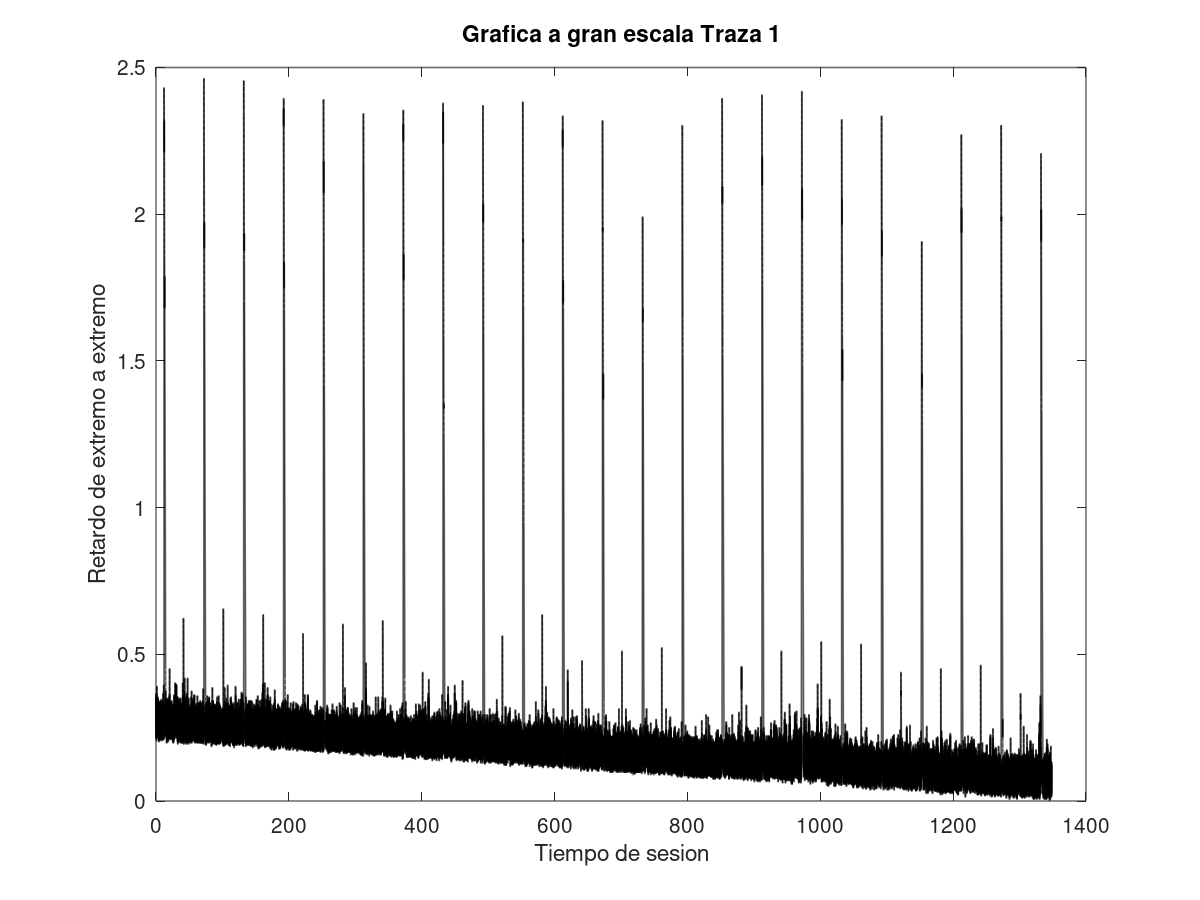
\includegraphics[width=0.45\textwidth]{img/traza1_GE.png}
      \hfill
      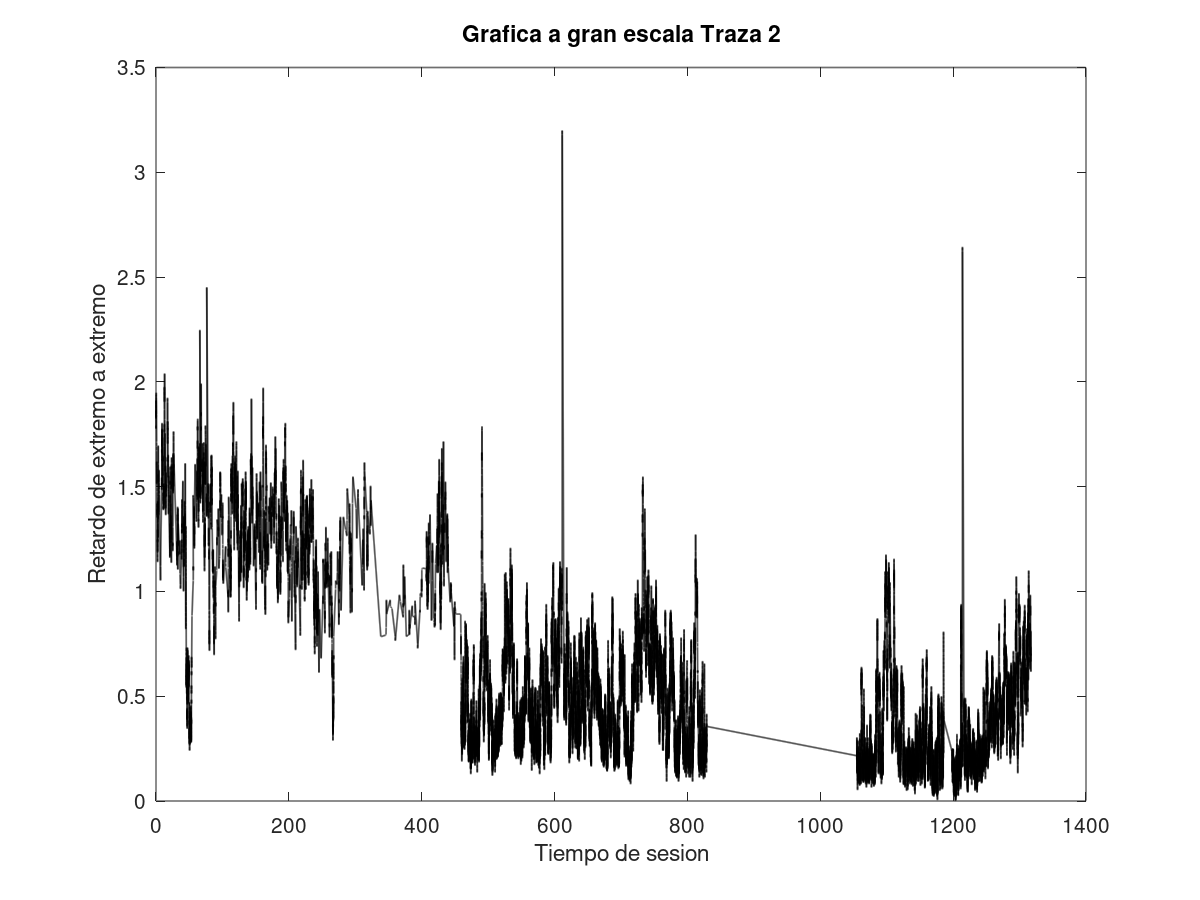
\includegraphics[width=0.45\textwidth]{img/traza2_GE.png}
      \vfill
      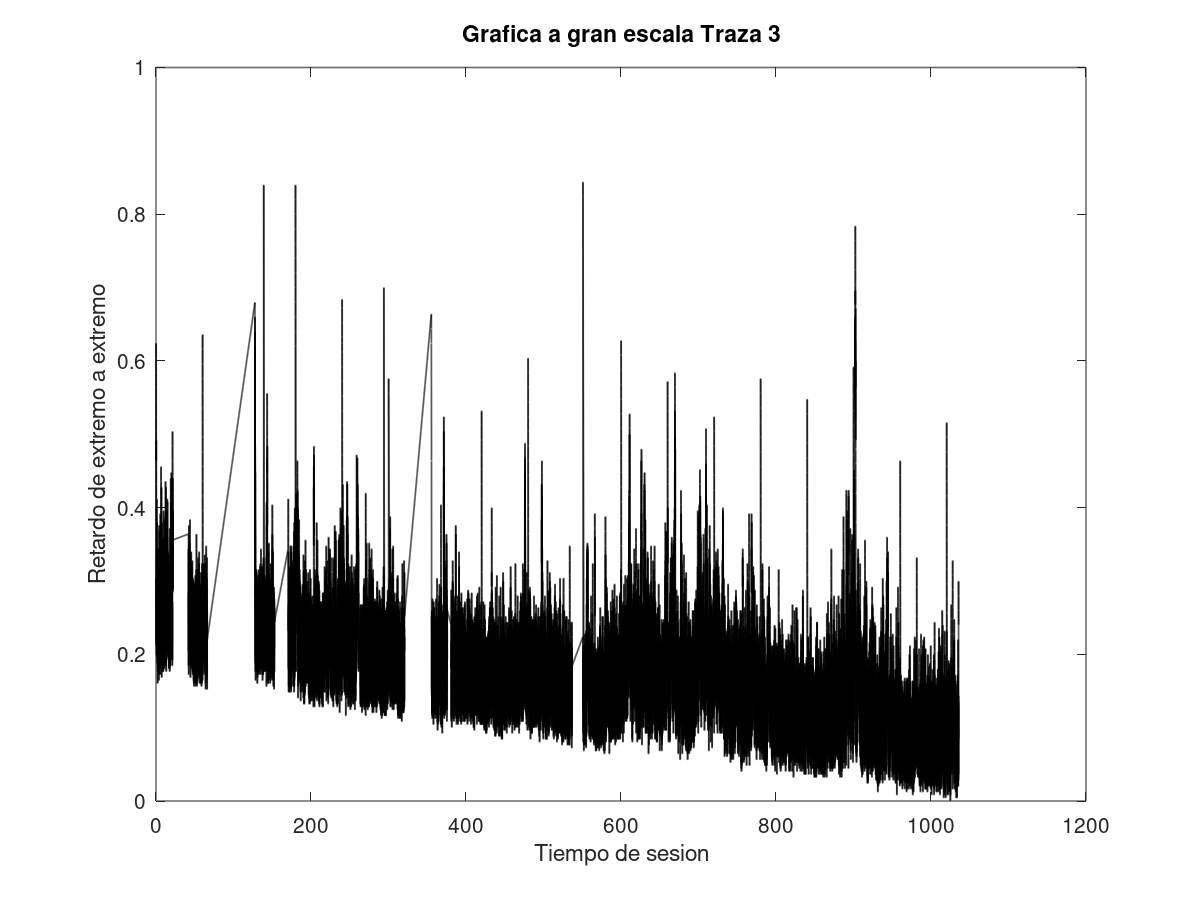
\includegraphics[width=0.45\textwidth]{img/traza3_GE.png}
      \hfill
      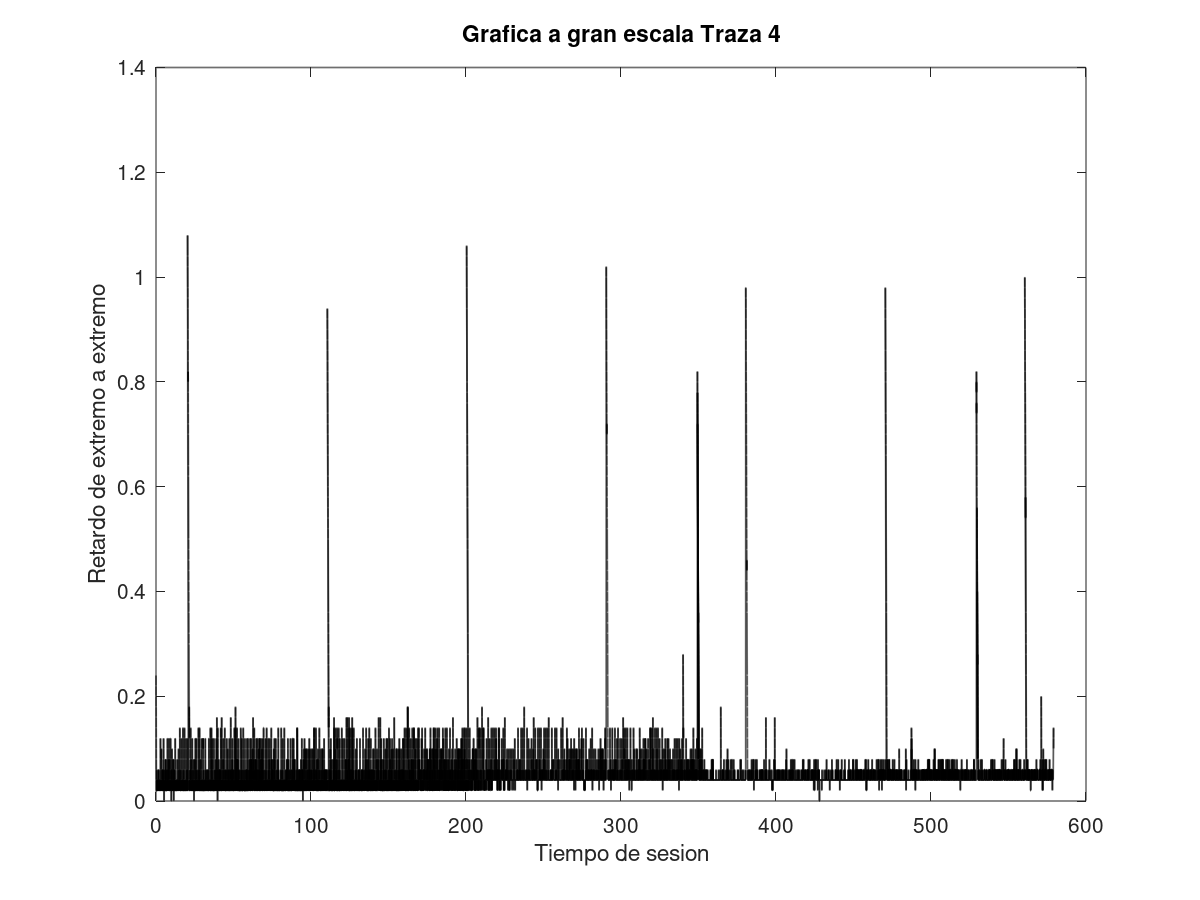
\includegraphics[width=0.45\textwidth]{img/traza4_GE.png}
      \vfill
      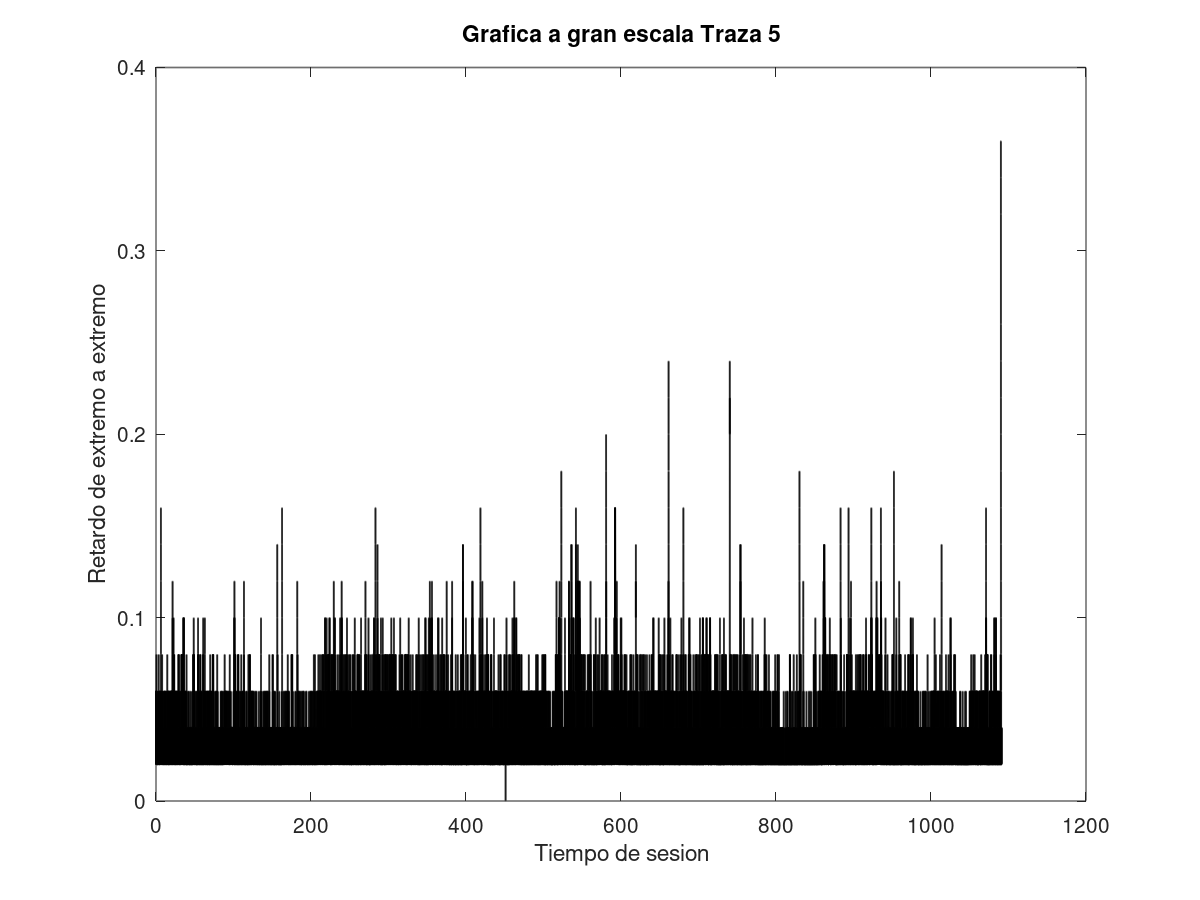
\includegraphics[width=0.45\textwidth]{img/traza5_GE.png}
      \hfill
      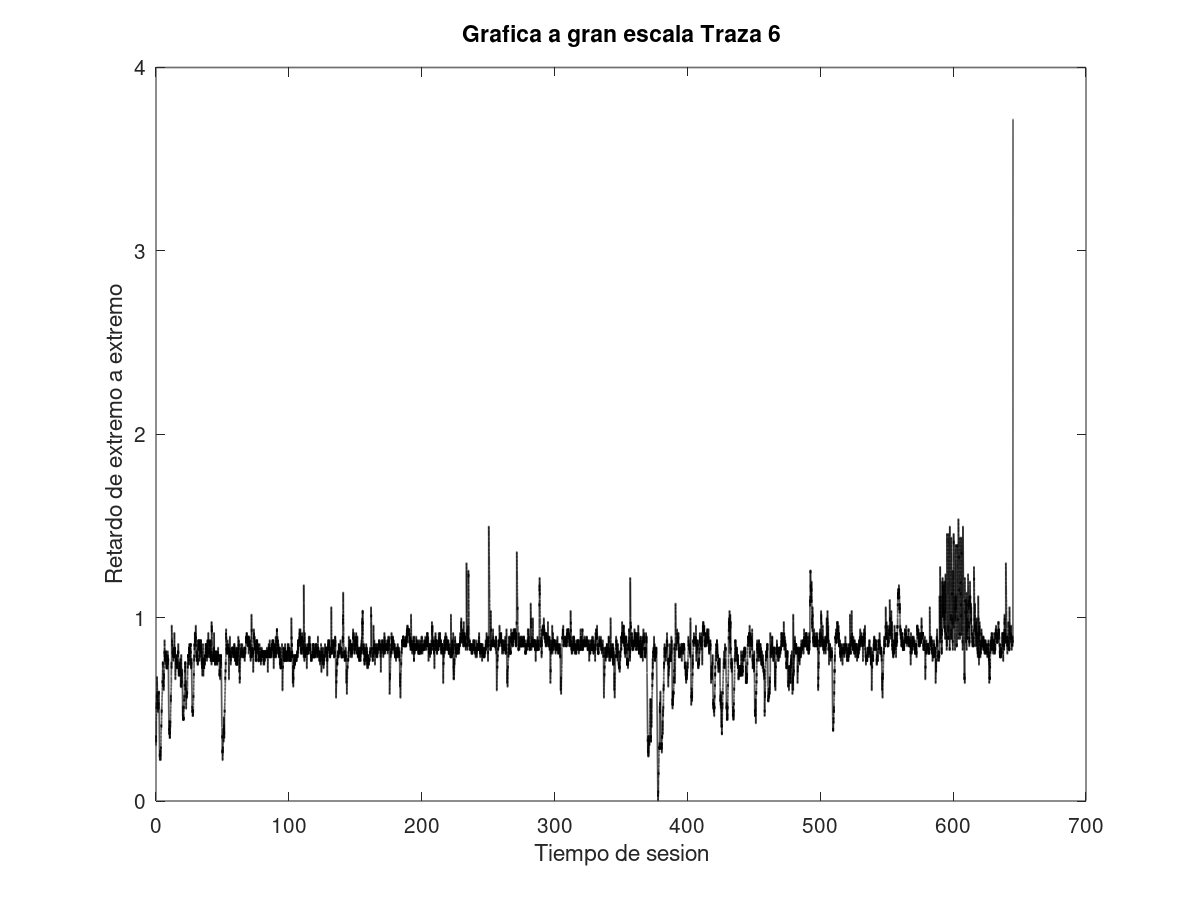
\includegraphics[width=0.45\textwidth]{img/traza6_GE.png}
      \vfill
  \end{figure}


  \item Gr\'aficas a pequeña escala. Se trazan dos o tres frases en la conversaci\'on.
  \noindent El primer paso para poder trazar las gr\'aficas a pequeña escala es acotar las sesiones a unas cuantas frases. Para esto
  usaremos el siguiente script en AWK que solo obtiene los datos de las primeras cuatro frases
  \begin{figure}[H]
    \centering
    \begin{lstlisting}[frame=single, breaklines=true, basicstyle=\footnotesize\ttfamily, breakatwhitespace=false, 
      columns=flexible, tabsize=2, showstringspaces=false, language=AWK]

      # Este script genera un archivo con dos columnas: tiempo de la sesion y retardo extremo a extremo.
      BEGIN{
          #Llama al script que se encarga de obtener la diferencia minima
          temp_file = "output.tmp"
          input_file = ARGV[1]
          command = "awk -f ../Script_3/script3.awk "input_file " > " temp_file
          system(command)
      
          # Procesa la salida del archivo temporal
          while ((getline line < temp_file) > 0) {
              # Procesa cada linea de salida del segundo script
              if (line ~ /Diferencia minima:/) {
                  split(line, fields, ":")
                  tmin = fields[2]
              }
          }
      
          # Limpia el archivo temporal
          system("rm -f " temp_file)
      
          t1_flag = 0
          talkspurts = 1
      }
      
      $1 == "D"{
      
          if (t1_flag == 0){
              t1 = $3
              t1_flag = 1
          }
      
          session_time = ($3 - t1) / 8000
          end_to_end_delay = ($2 - $3 - tmin) / 8000
          print session_time, end_to_end_delay
      }
      
      
      $1 == "!"{
        talkspurts++ # Incrementa el contador al encontrar un espacio de silencio
        if(talkspurts == 11){
          exit # Termina la ejecucion si encuentra cuatro signos "!"
        }
      }
      
    \end{lstlisting}
  \end{figure}

  \noindent El siguiente paso es usar el siguiente script en Octave para poder trazar las gr\'aficas
  \begin{figure}[H]
    \centering
    \begin{lstlisting}[frame=single, breaklines=true, basicstyle=\footnotesize\ttfamily, breakatwhitespace=false, 
      columns=flexible, tabsize=2, showstringspaces=false]

      data = load('output1_PE.txt');
      x = data(:, 1);
      y = data(:, 2);
      stem (x,y, 'Color', 'k');
      xlabel ('Tiempo de sesion');
      ylabel ('Retardo de extremo a extremo');
      title ('Grafica a gran escala Traza 1');
      print -dpng "../../Reporte/img/traza1_PE.png";

    \end{lstlisting}
  \end{figure}

  \begin{figure}[H]
    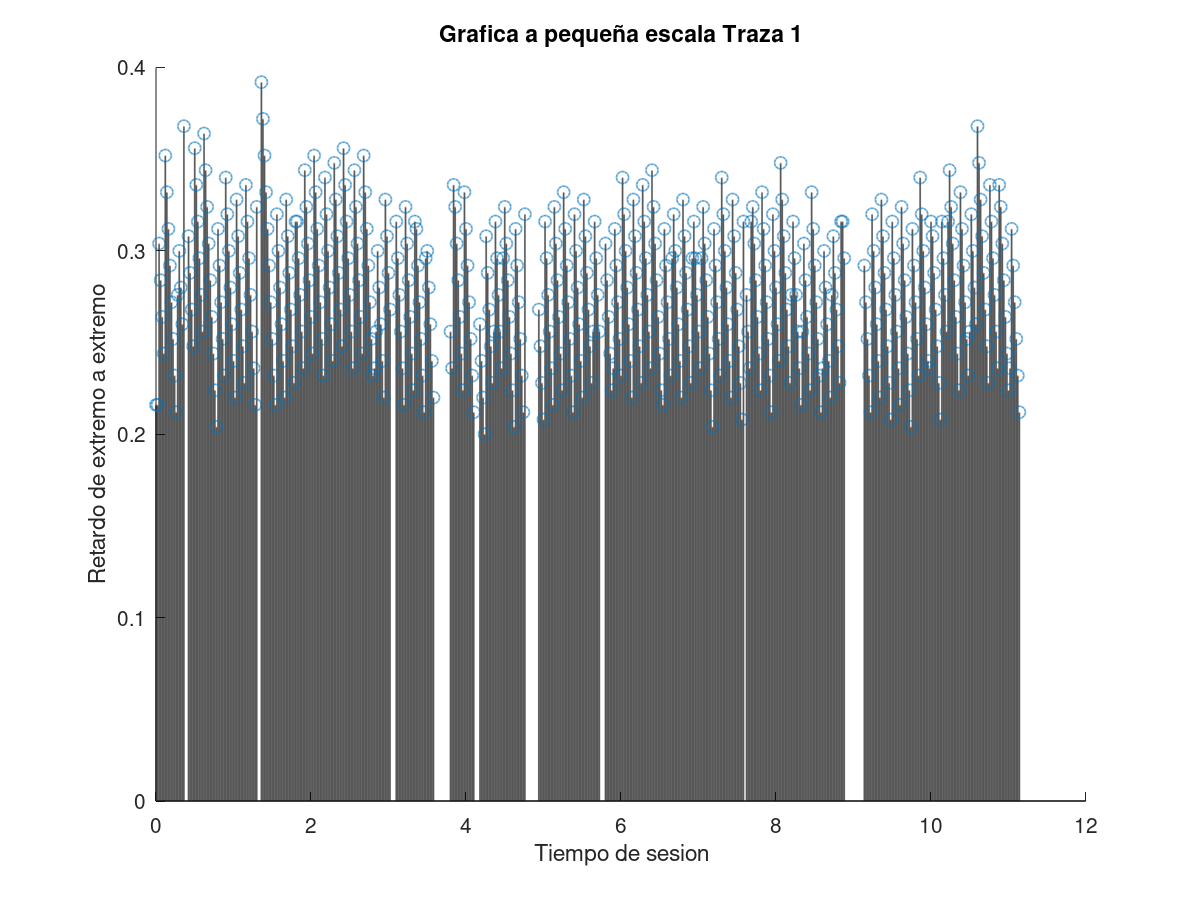
\includegraphics[width=0.45\textwidth]{img/traza1_PE.png}
    \hfill
    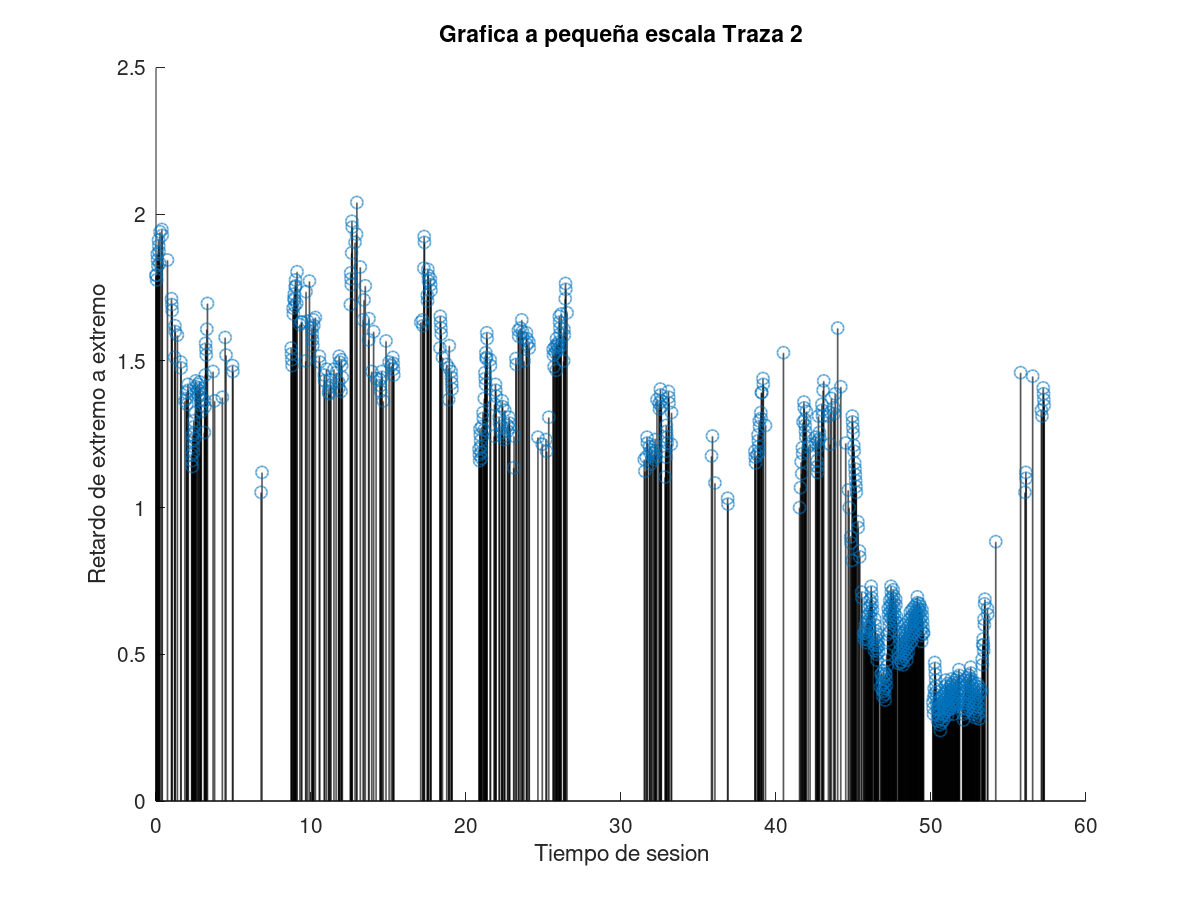
\includegraphics[width=0.45\textwidth]{img/traza2_PE.png}
    \vfill
    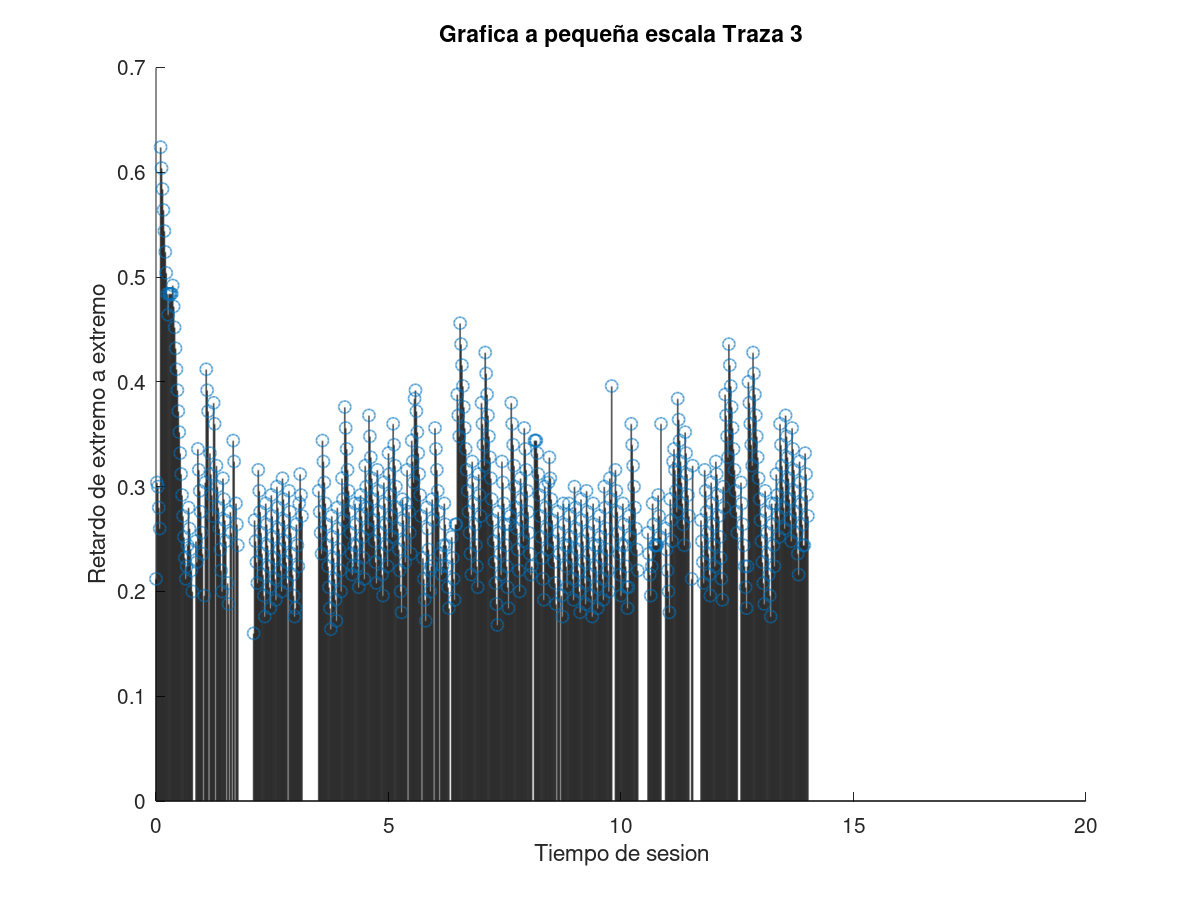
\includegraphics[width=0.45\textwidth]{img/traza3_PE.png}
    \hfill
    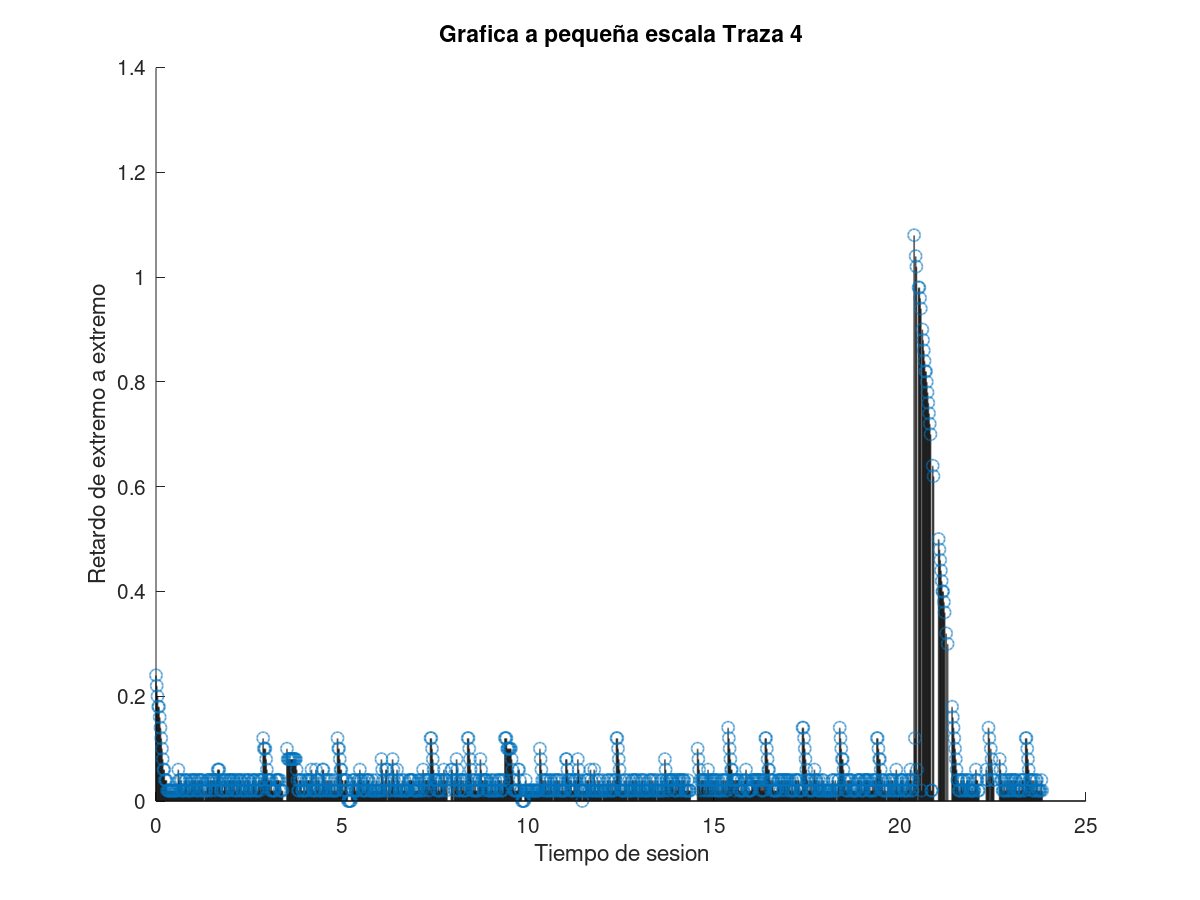
\includegraphics[width=0.45\textwidth]{img/traza4_PE.png}
    \vfill
    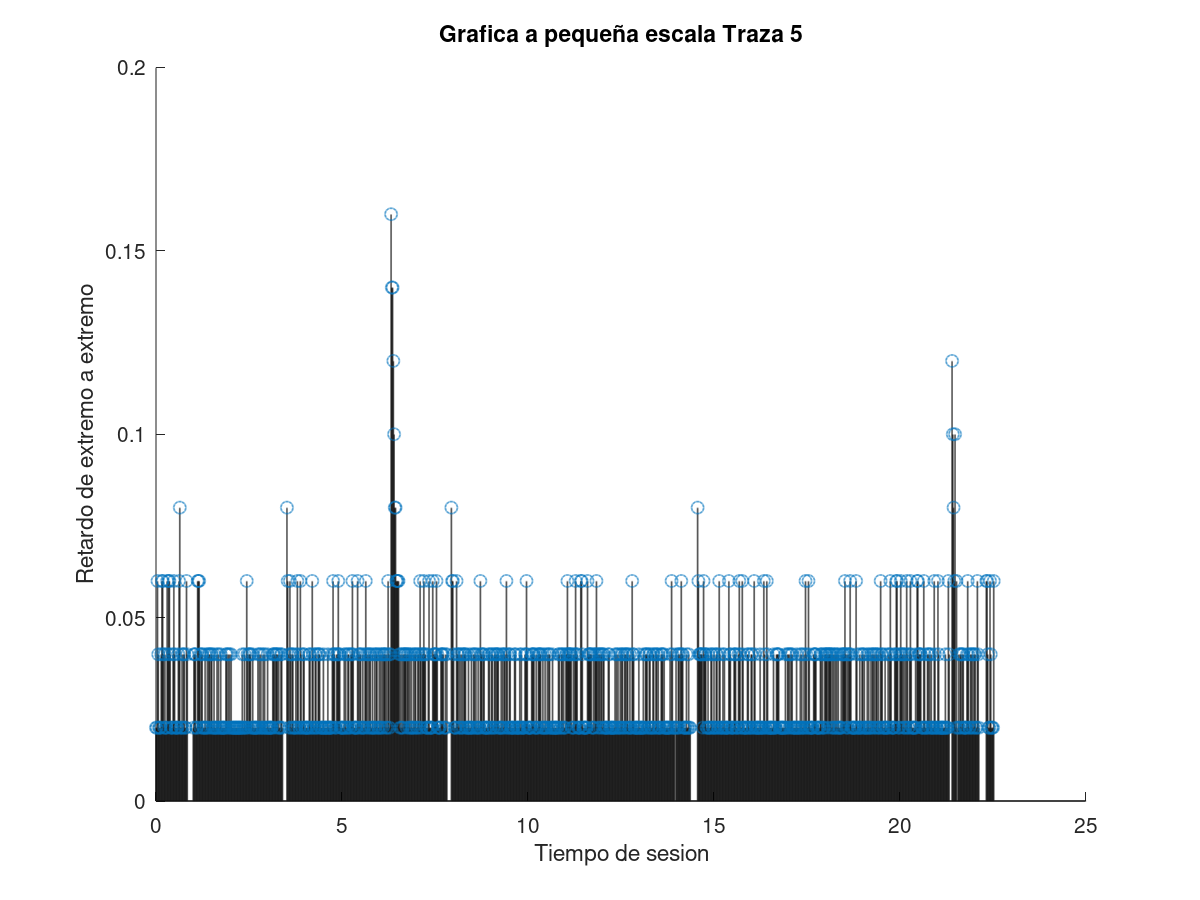
\includegraphics[width=0.45\textwidth]{img/traza5_PE.png}
    \hfill
    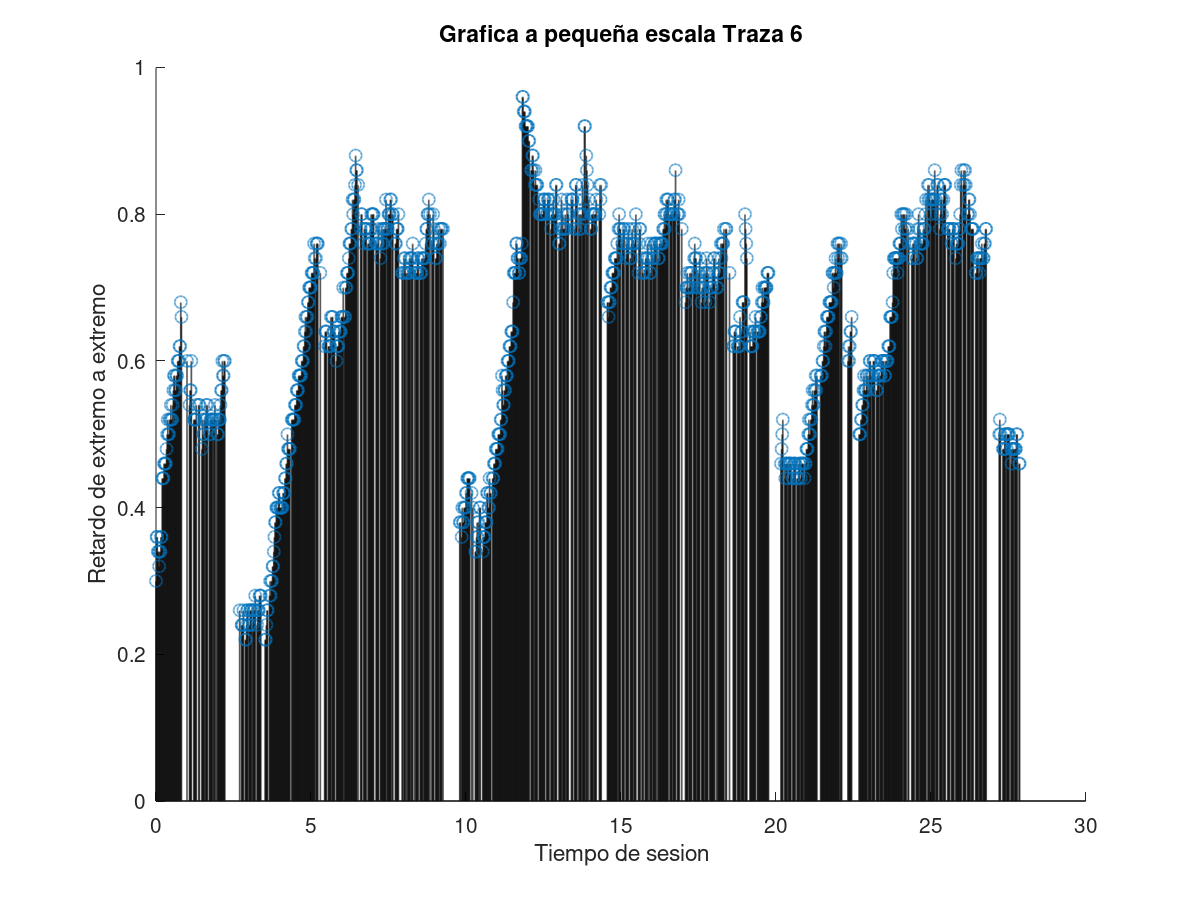
\includegraphics[width=0.45\textwidth]{img/traza6_PE.png}
    \vfill
\end{figure}

\item ¿C\'uales son los fen\'omenos particulares que observa usted en las gr\'aficas que acaba de obtener?
\noindent 

\item Tabla con las estad\'isticas obtenidas
\begin{table}[H]
  \centering
  \begin{tabular}{@{}ccccc@{}}
  \toprule
  \# Traza & \begin{tabular}[c]{@{}c@{}}Total de\\ frases\end{tabular} & \begin{tabular}[c]{@{}c@{}}Total de\\ paquetes\end{tabular} & \begin{tabular}[c]{@{}c@{}}Diferencia\\ mínima\end{tabular} & \begin{tabular}[c]{@{}c@{}}Retardo promedio\\ extremo a extremo\end{tabular} \\ \midrule
  1        & 818                                                       & 56,979                                                      & -641,808                                                    & 0.110536                                                                     \\
  2        & 406                                                       & 24,490                                                      & \multicolumn{1}{l}{-14,643,186}                             & 0.392336                                                                     \\
  3        & 536                                                       & 37,640                                                      & -774,206                                                    & 0.109097                                                                     \\
  4        & 252                                                       & 27,814                                                      & -807,010                                                    & 0.0486863                                                                    \\
  5        & 540                                                       & 52,836                                                      & -944,917                                                    & 0.0224502                                                                    \\
  6        & 299                                                       & 23,293                                                      & -1,489,551                                                  & 0.690046                                                                     \\ \bottomrule
  \end{tabular}
  \end{table}

  \item 
\end{enumerate}
\end{document}